\section{Технологическая часть}
\subsection{Требования к программному обеспечению}

\hspace{1.25cm}
На вход программе подаются 2 строки из символов, которые входят в таблицу Юникода (UTF-8).

На выход программа выдаёт число – расстояние между строками, вычисленное алгоритмом Левенштейна или Дамерау-Левенштейна матричной или рекурсивной реализацией. Для матричных реализаций также выводится матрица расстояний. Также в зависимости от выбранного пункта меню программа замеряет время работы алгоритмов и рисует получившиеся графики.

\subsection{Средства реализации}

\hspace{1.25cm}
Python эффективно обработывает строки и имеет богатую библиотеку, поэтому программа была реализована на этом языке программирования. Для замеров времени была использована функция \texttt{process\_time()} из библиотеки \texttt{time}, вычисляющая процессорное время\cite{process_time}.

\subsection{Реализации алгоритмов}

\hspace{1.25cm}
Ниже приведены листинги реализаций алгоритмов поиска расстояния Левенштейна и Дамерау-Левенштейна матричным, рекурсивным и рекурсивно-матричным способами на Python.

\vspace{0.25cm}
\begin{lstlisting}[caption=реализация матричного алгоритма Левенштейна]
def algo_Levenstein_matrix(str1: str, str2: str) -> int:
    len1, len2 = len(str1) + 1, len(str2) + 1
    if len2 > len1:
        str1, str2 = str2, str1
        len1, len2 = len2, len1
    old_str = [i for i in range(len2)]
    cur_str = [0 for _ in range(len2)]
    for i in range(1, len1):
        cur_str[0] = i
        for j in range(1, len2):
            cur_str[j] = min(cur_str[j - 1] + 1,
                            old_str[j] + 1,
                            old_str[j - 1] + (str1[i - 1] != str2[j - 1]))
        old_str = cur_str.copy()
    return cur_str[-1]
\end{lstlisting}

\vspace{0.25cm}
\begin{lstlisting}[caption=реализация рекурсивного алгоритма Левенштейна]
def algo_Levenstein_recursion(str1: str, str2: str) -> int:
    len1, len2 = len(str1), len(str2)
    if len1 * len2 == 0:
        return abs(len2 - len1)
    return min(algo_Levenstein_recursion(str1, str2[:-1]) + 1,
                algo_Levenstein_recursion(str1[:-1], str2) + 1,
                algo_Levenstein_recursion(str1[:-1], str2[:-1]) + (str1[-1] != str2[-1]))
\end{lstlisting}

\vspace{0.25cm}
\begin{lstlisting}[caption=реализация рекурсивно-матричного алгоритма Левенштейна]
def algo_Levenstein_recursion_matrix(str1: str, str2: str) -> int:
    len1, len2 = len(str1) + 1, len(str2) + 1
    mat = [[float("-inf") for i in range(len2)] for j in range(len1)]
    # the recursive part itself
    def recursion_part(str1: str, str2: str, mat: List[float] = []) -> int:
        len1, len2 = len(str1), len(str2)
        if mat[len1][len2] > float("-inf"):
            pass
        elif len1 * len2 == 0:
            mat[len1][len2] = abs(len2 - len1)
        else:
            mat[len1][len2] = min(recursion_part(str1, str2[:-1], mat) + 1,
                    recursion_part(str1[:-1], str2, mat) + 1,
                    recursion_part(str1[:-1], str2[:-1], mat) + (str1[-1] != str2[-1]))
        return mat[len1][len2]
    return recursion_part(str1, str2, mat)
\end{lstlisting}

\vspace{0.25cm}
\begin{lstlisting}[caption=реализация матричного алгоритма Дамерау-Левенштейна]
def algo_Damerau_Levenstein_matrix(str1: str, str2: str) -> int:
    len1, len2 = len(str1) + 1, len(str2) + 1
    if len2 > len1:
        str1, str2 = str2, str1
        len1, len2 = len2, len1
    old_str = [i for i in range(len2)]
    cur_str = [0 for _ in range(len2)]
    for i in range(1, len1):
        cur_str[0] = i
        for j in range(1, len2):
            m = str1[i - 1] != str2[j - 1]
            cur_str[j] = min(cur_str[j - 1] + 1,
                            old_str[j] + 1,
                            old_str[j - 1] + m)
            if (i > 1) and (j > 1) and m and (str1[i - 2] == str2[j - 1]) and (str1[i - 1] == str2[j - 2]):
                cur_str[j] = min(cur_str[j], old_str[j - 1])
        old_str = cur_str.copy()
    return cur_str[-1]
\end{lstlisting}

\vspace{0.25cm}
\begin{lstlisting}[caption=реализация рекурсивного алгоритма Дамерау-Левенштейна]
def algo_Damerau_Levenstein_recursion(str1: str, str2: str) -> int:
    len1, len2 = len(str1), len(str2)
    if len1 * len2 == 0:
        return abs(len2 - len1)
    res = min(algo_Damerau_Levenstein_recursion(str1, str2[:-1]) + 1,
                algo_Damerau_Levenstein_recursion(str1[:-1], str2) + 1,
                algo_Damerau_Levenstein_recursion(str1[:-1], str2[:-1]) + (str1[-1] != str2[-1]))
    if ((len(str1) >= 2) and (len(str2) >= 2) and (str1[-1] == str2[-2]) and (str1[-2] == str2[-1])):
        res = min(res, algo_Damerau_Levenstein_recursion(str1[:-2], str2[:-2]) + 1)
    return res
\end{lstlisting}

\vspace{0.25cm}
\begin{lstlisting}[caption=реализация рекурсивно-матричного алгоритма Дамерау-Левенштейна]
def algo_Damerau_Levenstein_recursion_matrix(str1: str, str2: str) -> int:
    len1, len2 = len(str1) + 1, len(str2) + 1
    mat = [[float("inf") for i in range(len2)] for j in range(len1)]
    # the recursive part itself
    def recursion_part(str1: str, str2: str, mat: List[float] = []) -> int:
        len1, len2 = len(str1), len(str2)
        if mat[len1][len2] < float("inf"):
            pass
        elif len1 * len2 == 0:
            mat[len1][len2] = abs(len2 - len1)
        else:
            mat[len1][len2] = min(recursion_part(str1, str2[:-1], mat) + 1,
                    recursion_part(str1[:-1], str2, mat) + 1,
                    recursion_part(str1[:-1], str2[:-1], mat) + (str1[-1] != str2[-1]))
            if ((len(str1) >= 2) and (len(str2) >= 2) and (str1[-1] == str2[-2]) and (str1[-2] == str2[-1])):
                mat[len1][len2] = min(mat[len1][len2], recursion_part(str1[:-2], str2[:-2], mat) + 1)
        return mat[len1][len2]
    return recursion_part(str1, str2, mat)
\end{lstlisting}

\vspace{0.25cm}
\subsection{Тесты}

Для тестирования алгоритмов Левенштейна и Дамерау-Левенштейна были составлены таблицы с входными данными (2 строки, возможно, пустые - $\lambda$), ожидаемым результатом (расстоянием) и полученным результатом от всех трёх способов.

\begin{table}[H]
    \centering
    \begin{tabular}{|c|c|c|c|c|c|}
        \hline
        \textbf{Строка 1} & \textbf{Строка 2} & \textbf{Ожидание} & \textbf{матричный} & \textbf{рекурсивный} & \makecell{\textbf{рекурсивно-}\\\textbf{матричный}} \\
        \hline
        $\lambda$ & $\lambda$ & 0 & 0 & 0 & 0 \\
        a  & a  & 0 & 0 & 0 & 0 \\
        abc & abc & 0 & 0 & 0 & 0 \\
        $\lambda$  & a  & 1 & 1 & 1 & 1 \\
        a  & $\lambda$  & 1 & 1 & 1 & 1 \\
        a  & b  & 1 & 1 & 1 & 1 \\
        abc & abs & 1 & 1 & 1 & 1 \\
        odc & abc & 2 & 2 & 2 & 2 \\
        ods & abc & 3 & 3 & 3 & 3 \\
        abcs & abc & 1 & 1 & 1 & 1 \\
        bc & abc & 1 & 1 & 1 & 1 \\
        bac & abc & 2 & 2 & 2 & 2 \\
        \hline
    \end{tabular}
    \caption{Таблица тестов для алгоритмов Левенштейна}
\end{table}

\begin{table}[H]
    \centering
    \begin{tabular}{|c|c|c|c|c|c|}
        \hline
        \textbf{Строка 1} & \textbf{Строка 2} & \textbf{Ожидание} & \textbf{матричный} & \textbf{рекурсивный} & \makecell{\textbf{рекурсивно-}\\\textbf{матричный}} \\
        \hline
        $\lambda$ & $\lambda$ & 0 & 0 & 0 & 0 \\
        a  & a  & 0 & 0 & 0 & 0 \\
        abc & abc & 0 & 0 & 0 & 0 \\
        $\lambda$  & a  & 1 & 1 & 1 & 1 \\
        a  & $\lambda$  & 1 & 1 & 1 & 1 \\
        a  & b  & 1 & 1 & 1 & 1 \\
        abc & abs & 1 & 1 & 1 & 1 \\
        odc & abc & 2 & 2 & 2 & 2 \\
        ods & abc & 3 & 3 & 3 & 3 \\
        abcs & abc & 1 & 1 & 1 & 1 \\
        bc & abc & 1 & 1 & 1 & 1 \\
        bac & abc & 1 & 1 & 1 & 1 \\
        \hline
    \end{tabular}
    \caption{Таблица тестов для алгоритмов Дамерау-Левенштейна}
\end{table}

В ходе проведённого тестирования (с помощью pytest) ошибок в алгоритмах не выявлено (см. Рис.~\ref{fig:pytest_result}).\\[0.1cm]

\begin{figure}[H]  % Принудительное размещение изображения
    \centering
    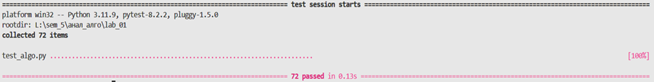
\includegraphics[width=1\textwidth]{img/pytest_result.png}
    \caption{Результаты тестов с использованием pytest}
    \label{fig:pytest_result} % Метка для ссылки на картинку
\end{figure}

\newpage